\section{Hybrid Model Architecture}
\label{section:Architecture:Model}

We propose a prediction framework based on the one presented in \cite{Zhao2019}.
Creating a Convolutional autoencoder and LSTM method for time-series prediction should provide some benefits.
Primarily, the combination of methods should help with increasing the prediction accuracy in data with high fluctuations.
Unlike the univariate method used in \cite{Zhao2019},
% we intend to improve upon the method by applying it as a global method and a multivariate method.
we intend to improve upon the method by experimenting with different model structures to capture interdependent relationships in a time-series cluster.
Such a method has never been explored in the E-commerce forecasting domain, warranting the exploration of the method's applicability to the problem space.
% Add explainer to why we do this?
% Add line as to explain that this is a new method in E-commerce forecasting?

The proposed framework is comprised of two parts: the convolutional autoencoder and the LSTM.

The convolutional autoencoder process the input data, extracting a feature set by deconstructing the data.
This is done through the encoder. After this, the decoder is used to reconstruct the input data.
By doing this, the noise in the input data should be decreased to some extent.

The second part of the architecture is the LSTM module.
This module is intended to extract the temporal features of the dataset
to predict future values in the time-series.

\begin{figure}[h!]
  \centering
  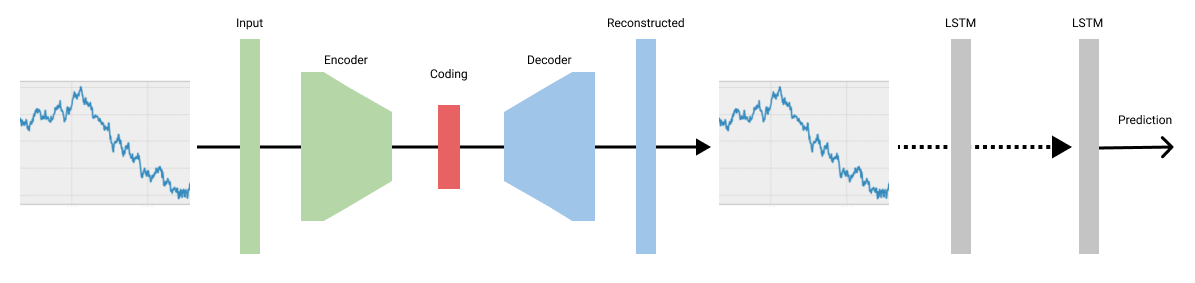
\includegraphics[width=\textwidth]{./figs/illustrations/CNN-AE + LSTM.png}
  \hfill
  \caption{Illustration of a CNN-AE + LSTM network.}
  \label{fig:cnn-ae+lstm-network}
\end{figure}

Finally, the complete framework proposed in this paper connects these two models,
creating a convolutional autoencoder and LSTM framework for making predictions.
These predictions are intended to function on time-series data with high fluctuations,
making accurate and less error-prone predictions than simple statistical or deep learning methods.


As a means to validate the proposed method, predictive benchmarks should be provided.
Established methods such as the SARIMA method and the LSTM method are well suited for this.
These methods create a baseline that can be used to establish the comparative performance with the proposed method.

The motivation behind the proposed framework is explored in further detail later in \Cref{section:Discussion}.



\subsection{The Auto-encoder}

The first part of the proposed hybrid model is the convolutional autoencoder used to process the input data.
As described, the task of the autoencoder is to encode and reconstruct the input data,
while decreasing the noise.

The design of the autoencoder is based on the paper by \cref{Zhao2019},
detailing a convolutional autoencoder comprised only of 1 dimensional convolutional and trans-convolutional layers.

% How was the selected model comprised?
% Why do we not use max pooling?
% Why do we not use dropout?
% Why do we not use batch normalization?
% Why do we not use fully connected layers?

In order to find a well-suited autoencoder model for our problem-space,
we designed a model to reconstruct the input data with high accuracy,
while still removing noise from the dataset.
Due to the fact that all the data in the different datasets share similar characteristics
a shared autoencoder model is developed.

The autoencoder consists of 4 layers, 2 encoder layers, and 2 decoder layers.
The encoder is created as two 1-dimensional convolutional layers with an increasing number of filters.
With a kernel size of [3, 5], and filter size if [16, 32].
The decoder is constructed similarly with two layers, where both are 1-dimensional trans-convolutional layers
with kernel size [5, 3] and a number of filters [16, 1].
The autoencoder layers do not contain any dropout.


While the autoencoder does contain convolutional and trans convolutional layers,
there are other aspects of the model that are not used.
Methods such as batch-normalization and MaxPooling is not used.
This is because adding these measures results in quite poor reconstructive results.
This is likely because of the high volatility of the data.
Other layers, such as the dense, fully connected layers, which often represent the coding in the autoencoder,
is not used either.
This is because it was found to be an unneeded increase in the complexity of the model,
as the convolutional layers were well suited to solve the task on their own.


There are two reasons for this.
Primarily this is due to the fact that during experimentation with the autoencoder models architecture,
it was found that the same autoencoder performed similarly on each of the individual time series.
Secondly, this was a decision that was made in connection with the limited time available for experimentation and optimization of models.



\subsection{LSTM}

The second part of the hybrid model is the LSTM model.
This model is attached at the end of the autoencoder,
using the reconstructed values from the autoencoder as input data.

% What can be said about the LSTM?
% Add use of local and global methods such as the with the LSTM model



% TODO:
% Explain the use of univarite and multivariate models
% Explain the use of global and local models
